\usetikzlibrary{calc}
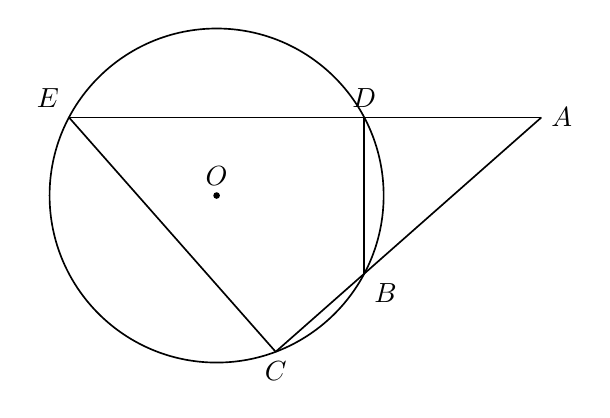
\begin{tikzpicture}[x=1cm,y=1cm,line width=.6pt,font=\normalsize]
\coordinate (E) at (-3.75,0);
\coordinate (D) at (0,0);
\coordinate (A) at (2.25,0);
\coordinate (B) at (0,-1.9843);
\coordinate (C) at (-1.125,-2.9765);
\coordinate (O) at (-1.875,-0.9922);
\draw[black] (O) circle[radius=2.1213cm];
\fill[black] (O) circle[radius=1.2pt];
\draw[black] (E)--(A);
\draw[black] (D)--(B);
\draw[black] (A)--(C);
\draw[black] (E)--(C);
\node[above left] at (E) {$E$};
\node[above] at (D) {$D$};
\node[right] at (A) {$A$};
\node[below right] at (B) {$B$};
\node[below] at (C) {$C$};
\node[above] at (O) {$O$};
\end{tikzpicture}
